\section{实验分析}
为了验证所提出的PermLLM方法,我们在不同的设定下进行了实验,包括了不同的网络环境以及不同的Transformer模型大小。
%
我们采用Pyfhel库~\cite{ibarrondo_2021_pyfhel}实现BFV同态加密,使用Pytorch~\cite{2019_pytorch}进行浮点运算,并采用Python原生套接字进行各方的网络通信。
%
我们的当前最新的基于密码学的大语言模型或Transformer模型隐私推断框架进行了对比,包括MPCFormer~\cite{li2022mpcformer}和Puma~\cite{dong2023puma}。
%
这些实验在搭载4张NVIDIA RTX 3090 (24G)显卡的服务器上进行。
%
此外,我们使用PermLLM框架实现了ChatGLM-6B模型~\cite{zeng_2022_glm130b},并在搭载有3台NVIDIA L20 (48G)的显卡的服务器上进行了实验。
%

我们考察了以下的网络环境:
\begin{itemize}
    \item LAN (Local Area Network):此时我们经由本机IP地址(127.0.0.1/localhost)进行通信,而未进行实际的网络通信。
    \item WAN1:往返时延为10ms,相当于400千米距离的网络时延,如东京到大阪;网络带宽为1Gbps,对应商用水平的网络连接。
    \item WAN2:往返时延为20ms,相当于1000千米距离的网络时延,如柏林到伦敦;网络带宽为100Mbps,对应家用网络。
\end{itemize}


\subsection{基准测试}
我们首先对非线性函数计算和单层的Transformer推断进行了基准测试,并且测量了通信量、通信轮数和总的执行时间。
我们将非线性函数的结果汇报在\autoref{tab:perm-llm:nonlinear}中,将单层Transformer结果汇报在\autoref{tab:perm-llm:layer}中。
%
表中LN表示层归一化,Any表示任意非线性函数。
%
\begin{table}[h!]
    \small
    \caption{非线性函数的基准测试}
    \label{tab:perm-llm:nonlinear}
    \begin{tabular}{@{}cccrrrrr@{}}
    \toprule
    $f$ & $n$ & 方法 & 通信(Mb) & 轮数 & LAN & 1Gbps/10ms & 100Mbps/20ms \\ \midrule
    \multirow{6}{*}{\parbox[t]{2mm}{\multirow{3}{*}{\rotatebox[origin=c]{90}{Argmax}}}} & \multirow{3}{*}{1K} & MPCFormer & 1.24 & 101 & 0.09 ± 0.01 & 2.11 ± 0.00 & 4.12 ± 0.01 \\ \cmidrule(l){3-8} 
     &  & Puma & $\approx$0.80 & $\approx$1700 & 0.15 ± 0.03 & 3.29 ± 0.03 & 6.33 ± 0.05 \\ \cmidrule(l){3-8} 
     &  & \textbf{PermLLM} & \textbf{0.26} & \textbf{4} & \textbf{0.03 ± 0.00} & \textbf{0.05 ± 0.00} & \textbf{0.06 ± 0.01} \\ \cmidrule(l){2-8} 
     & \multirow{3}{*}{100K} & MPCFormer & 110.9 & 153 & 0.78 ± 0.04 & 4.04 ± 1.41 & 10.74 ± 0.50 \\ \cmidrule(l){3-8} 
     &  & Puma & $\approx$80 & $\approx$2500 & 1.17 ± 1.13 & 6.23 ± 0.08 & 12.88 ± 0.06 \\ \cmidrule(l){3-8} 
     &  & \textbf{PermLLM} & \textbf{4.02} & \textbf{4} & \textbf{0.12 ± 0.01} & \textbf{0.17 ± 0.01} & \textbf{0.2 ± 0.00} \\ \midrule
    \multirow{6}{*}{\parbox[t]{2mm}{\multirow{3}{*}{\rotatebox[origin=c]{90}{Element-wise}}}} & \multirow{3}{*}{1K} & Puma: GeLU & $\approx$1.7 & $\approx$200 & 0.04 ± 0.02 & 0.38 ± 0.02 & 0.71 ± 0.01 \\ \cmidrule(l){3-8} 
     &  & Puma: LN & $\approx$0.20 & $\approx$200 & 0.02 ± 0.00 & 0.35 ± 0.01 & 0.67 ± 0.01 \\ \cmidrule(l){3-8} 
     &  & \textbf{PermLLM: Any} & \textbf{0.01} & \textbf{3} & \textbf{0.00 ± 0.00} & \textbf{0.02 ± 0.00} & \textbf{0.04 ± 0.01} \\ \cmidrule(l){2-8} 
     & \multirow{3}{*}{\begin{tabular}[c]{@{}c@{}}100K\\100$\times$1K\end{tabular}} & Puma: GeLU & $\approx$170 & $\approx$200 & 1.32 ± 0.11 & 1.69 ± 0.23 & 12.37 ± 0.08 \\ \cmidrule(l){3-8} 
     &  & Puma: LN & $\approx$20 & $\approx$200 & 0.13 ± 0.03 & 0.15 ± 0.02 & 0.83 ± 0.03 \\ \cmidrule(l){3-8} 
     &  & \textbf{PermLLM: Any} & \textbf{1.15} & \textbf{3} & \textbf{0.01 ± 0.00} & \textbf{0.03 ± 0.01} & \textbf{0.05 ± 0.00} \\ \bottomrule
    \end{tabular}
\end{table}


\begin{table}[h]
\small
\centering
\caption{单层Transformer的基准测试}
\label{tab:perm-llm:layer}
\begin{tabular}{@{}ccrrrrr@{}}
\toprule
模型大小 & 方法           & 通信(Mb)   & 轮数        & LAN                   & 1Gbps/10ms            & 100Mbps/20ms         \\ \midrule
\multirow{3}{*}{\begin{tabular}[c]{@{}c@{}} 大 \\ ($d=4096$)\end{tabular}} & MPCFormer & 3073.79 & 53 & 1.37 ± 0.01 & 26.15 ± 0.35 & 259.65 ± 0.36 \\ \cmidrule(l){2-7} 
            & Puma        & $\approx$33   & $\approx$1500 & 8.82 ± 0.09           & 11.45 ± 0.42         & 14.40 ± 0.65         \\ \cmidrule(l){2-7} 
            & \textbf{PermLLM} & \textbf{0.49} & \textbf{20}   & \textbf{0.04 ± 0.01}  & \textbf{0.12 ± 0.01} & \textbf{0.24 ± 0.00} \\ \midrule
\multirow{3}{*}{\begin{tabular}[c]{@{}c@{}} 小 \\ ($d=768$)\end{tabular}}  & MPCFormer & 108.32  & 53 & 1.29 ± 0.19 & 1.71 ± 0.01  & 10.29 ± 0.20  \\ \cmidrule(l){2-7} 
            & Puma         & $\approx$6    & $\approx$1000 & 0.46 ± 0.03           & 2.24 ± 0.03          & 3.97 ± 0.04          \\ \cmidrule(l){2-7} 
            & \textbf{PermLLM} & \textbf{0.1}  & \textbf{20}   & \textbf{0.03 ± 0.00} & \textbf{0.15 ± 0.01} & \textbf{0.23 ± 0.02} \\ \bottomrule
\end{tabular}
\end{table}

可以看到,对于非线性运算而言,在任意输出规模或网络环境下,PermLLM框架都达到了最高的效率,其通信轮数、通信量以及时间消耗都显著低于对比算法。
%
不同于对比算法需要针对特定的非线性函数设计安全计算协议,PermLLM框架通过随机排列的方法,任何逐元素非线性函数都能在3轮通信中完成计算。
%
同时,其通信量也只是明文大小的4倍。
%
对于Argmax函数,我们使用的基于同态加密的安全解码算法,只需要进行数十次同态乘法和同态加法,即可完成计算,其速度也大幅领先对比算法。

同样地,对于单层Transformer推断,PermLLM也达到了最大的效率。
%
且对于更大的Transformer,PermLLM的优势更大,说明了其在大语言模型中会具有更大的优势。
当Transformer的维度从768提升到4096后,其优势从一个数量级提升至两个数量级。
%
我们也注意到,在MPCFormer~\cite{li2022mpcformer}中,其采用Crypten框架~\cite{knott2021crypten}默认的算子进行秘密分享乘法,没有考虑到大语言模型的权重固定情况。
%
每一次秘密分享乘法时,都会对权重产生新的Beaver三元组并分发给$P_0$和$P_1$,以及恢复遮罩过的权重($X - U$),带来了巨大的额外性能损耗。


\subsection{ChatGLM-6B测试}
我们使用PermLLM框架实现了ChatGLM-6B模型~\cite{zeng_2022_glm130b},并且在两个WAN (Wide Area Network) 网络环境下进行了实验。
%
我们选择了6,15,37和62长度的输入文本,测量了每生成一个单词所需的时间和流量,绘制在\autoref{fig:perm-llm:chatglm}中。
%
可以看到,在WAN2(20ms/100Mbps)环境下,每个单词生成的时间大概在7秒左右;而在更快的WAN1(10ms/1Gbps)下,单词生成的时间仅需3秒左右。
%
注意到第一个单词产生的时间较长,这是因为在第一个单词生成时,要把整个输入文本放入模型进行推断;但是因为我们采用了键值缓存技术,之后只需要放入新生成的文本即可。
%
这个实验证明了PermLLM可以在普通的网络环境下把大模型隐私推断的时间提升到秒级别,相比于现有的密码学方案提升了两个数量级以上,从而使其具备一定的实用性。
%
此外,若在相同配置下进行单机的ChatGLM6B推断,其速度大概为0.1s/词,因此PermLLM在文本生成时,依然需要花费单机推断数十倍的时间。


\begin{figure}[htbp]
    \centering
    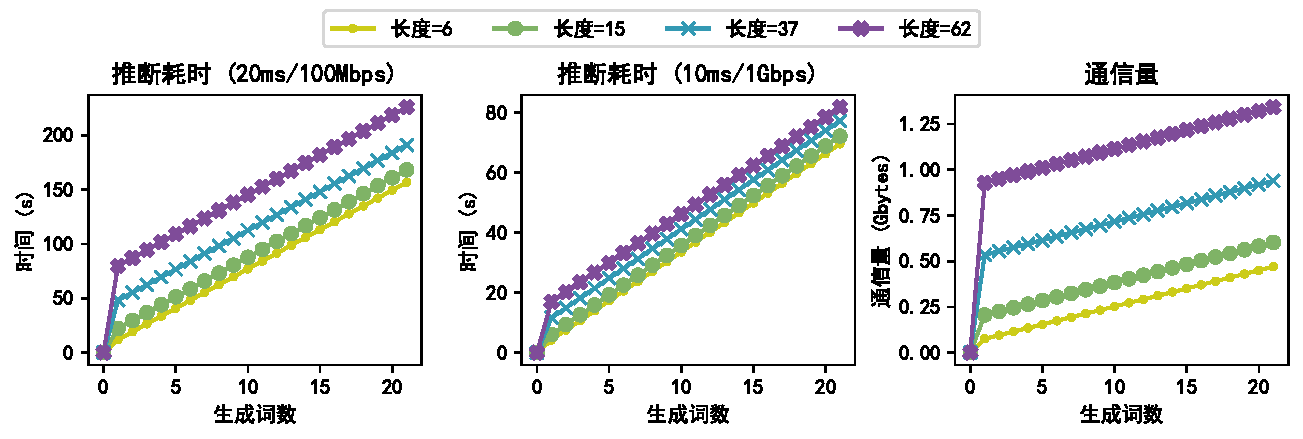
\includegraphics[width=\linewidth]{Z_Resources/perm-llm_ChatGLM.pdf}
    \caption{ChatGLM-6B实验结果}
    \label{fig:perm-llm:chatglm}
\end{figure}


此外,实验也观察到PermLLM框架几乎不会有准确率的损失。
%
这是因为浮点秘密分享的情况下,误差来源仅为秘密分享计算中的浮点计算舍入误差(Rounding Error)。
%
即使将其转化为整数计算,只需要设置精度位,同样可以实现几乎无误差的隐私推断。
%
对比之下,基于密码学的方法由于采用了多项式拟合GeLU等技术,会带来除去舍入误差之外的更大误差。